\gdef\thisproblemauthor{Иван Казменко}
\gdef\thisproblemdeveloper{Иван Казменко}
\begin{problem}{Игра в покрытие}
{covering-game.in}{covering-game.out}
{2 секунды (\textsl{3 секунды для Java})}{256 мебибайт}{}

\begin{tabular}{lr}
\hskip -0.8cm
\begin{minipage}{0.70\thelinewidth}
\parindent=0.6cm
\textit{Дискретная трямая} "--- это аналог дискретной прямой,
состоящей из точек с целыми координатами.
Отличие состоит в том, что из каждой точки есть не два,
а три направления движения.
Дискретную трямую можно удобно изобразить на плоскости так, как это
показано на рисунке 1.

\textit{Расстояние} на дискретной трямой между точками $A$ и $B$ "--- это
минимальное количество переходов от точки к соседней, которое необходимо
сделать, чтобы попасть из точки $A$ в точку $B$.
Например, на рисунке 2 расстояние между точками $A$ и $B$ равно $5$.

\textit{Круг} на дискретной трямой радиуса $r$ с центром
в точке $T$ "--- это множество, состоящее изо всех точек трямой,
удалённых от $T$ не более, чем на расстояние $r$.
На рисунке 3 показаны примеры трёх кругов.
Их центры обозначены заглавными буквами, а остальные принадлежащие им
точки "--- соответствующими строчными буквами.

\textit{Отрезок} дискретной трямой "--- это, как и в случае прямой,
любая конечная связная фигура на дискретной трямой.
Такой отрезок можно интерпретировать как изображённый на плоскости граф,
являющийся деревом, в котором степень каждой вершины не превосходит трёх,
а соседние рёбра образуют углы, кратные 120 градусам.
Пример отрезка представлен на рисунке 4.

Будем задавать отрезок \textit{левым обходом} соответствующего ему дерева
из одного из его \textit{листьев}, то есть вершин, у которых ровно один сосед
в этом отрезке.
Если листьев в дереве нет, то оно состоит из одной вершины,
а его левый обход не содержит переходов.
В общем же случае объявим лист, из которого мы начали обход,
\textit{корнем} дерева.
Теперь у каждой вершины, кроме корня, есть \textit{предок} "--- та
из соседних вершин, которая ближе к корню дерева.

Левый обход дерева строится рекурсивно следующим образом.
Пусть мы находимся в вершине $v$ и смотрим в том же направлении,
вдоль которого мы в неё шли из предка (рисунок 5).
Если есть ребро из этой вершины вперёд и налево, пройдём по нему,
рекурсивно построим обход из вершины, в которую пришли,
после чего вернёмся в вершину $v$.
Далее, если есть ребро из этой вершины вперёд и направо, пройдём по нему
и также рекурсивно построим обход из вершины, в которую пришли,
после чего вернёмся в вершину $v$.
Поскольку в корне направление из предка не задано, условимся единственное
ребро из корня считать левым.

Будем использовать символ <<\t{l}>> для обозначения движения вперёд и налево,
символ <<\t{r}>> для движения вперёд и направо и
символ <<\t{b}>> для движения назад к корню.
Для примера запишем отрезок, представленный на рисунке 4.
Объявим корнем самый верхний лист, обозначенный буквой $A$.
Запись будет выглядеть так: <<\t{lllbrbbrlllbrbbrllbbrbbbrrbbbb}>>.
\end{minipage}
&
\begin{minipage}{0.27\thelinewidth}
\begin{center}
\vskip -70pt

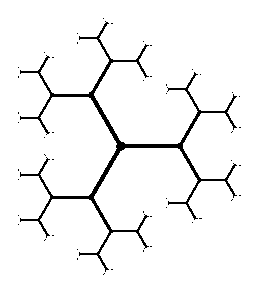
\includegraphics{covering-game.1.eps}

Рисунок 1

~

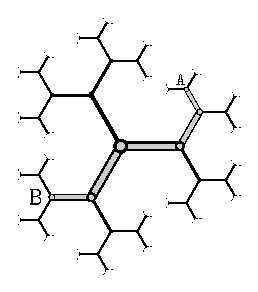
\includegraphics{covering-game.2.eps}

Рисунок 2

~

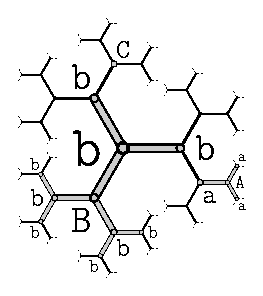
\includegraphics{covering-game.3.eps}

Рисунок 3

~

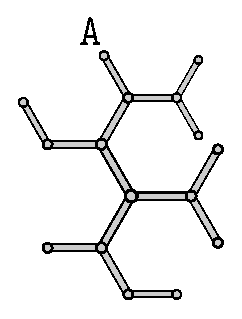
\includegraphics{covering-game.4.eps}

Рисунок 4

~

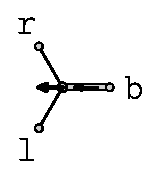
\includegraphics{covering-game.5.eps}

Рисунок 5
\end{center}
\end{minipage}
\end{tabular}

\newpage

Алиса, Боб и Карл играют в игру на дискретной трямой.
Сначала фиксируется игровое поле "--- некоторый отрезок дискретной трямой.
Игра заканчивается, когда все точки игрового поля оказываются покрыты;
изначально все точки считаются не покрытыми.
Игроки ходят по очереди: первой ходит Алиса, вторым "--- Боб,
а третьим "--- Карл.
Ход состоит в выборе точки на отрезке, которая ещё не покрыта.
После этого с центром в этой точке строится круг.
Радиус этого круга "--- максимальное целое неотрицательное число такое, что
все точки этого круга являются точками игрового поля и при этом ещё не покрыты.
Наконец, все точки этого круга объявляются покрытыми.
Проигрывает один из трёх игроков "--- тот, кто не может сделать очередной ход.

На рисунке 6 показано несколько позиций в игре и возможные ходы
из этих позиций.
Выбранная точка отмечена заглавной буквой, а другие точки круга,
который покрывается таким ходом "--- соответствующими прописными буквами.
Точки трямой, обведённые в двойной кружок "--- это покрытые ранее точки.
Помните, что центр круга игрок может выбирать, но после этого радиус
выбрать нельзя: он должен быть максимально возможным для этого центра
в текущей игровой ситуации.

\begin{center}
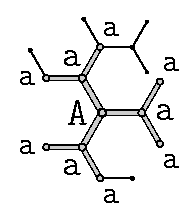
\includegraphics{covering-game.6.eps}
~~~~~
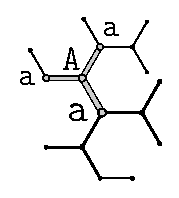
\includegraphics{covering-game.7.eps}
~~~~~
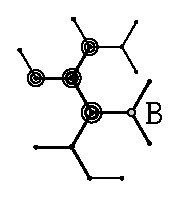
\includegraphics{covering-game.8.eps}
~~~~~
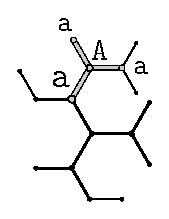
\includegraphics{covering-game.9.eps}
~~~~~
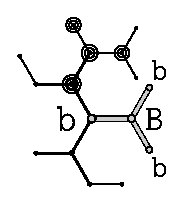
\includegraphics{covering-game.10.eps}

Рисунок 6
\end{center}

Кого из игроков можно заставить проиграть в этой игре?
Игрока $X$ можно заставить проиграть, если два других игрока могут
сговориться и действовать сообща так, чтобы $X$ не мог не проиграть.

\InputFile

В первой строке ввода задано целое число $m$ "--- количество символов
в строке, задающей левый обход игрового поля.
Во второй строке записаны $m$ символов без пробелов "--- левый обход
игрового поля.
Гарантируется, что этот левый обход корректно задаёт отрезок дискретной трямой,
содержащий от $1$ до $100$ точек.

\OutputFile

Выведите три строки.
В первой строке укажите, можно ли заставить проиграть Алису,
во второй "--- Боба, а в третьей "--- Карла.
Каждая строка должна состоять из слова <<\t{Yes}>> в случае положительного
ответа и из слова <<\t{No}>> в случае отрицательного.

\Example

\begin{examplethree}
\exmp{%
6
llbrbb
}{%
No
Yes
No
}{%
\vskip 0pt
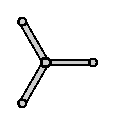
\includegraphics{covering-game.11.eps}
}%
\end{examplethree}

\Explanation

В этом простом примере у Алисы есть всего лишь два существенно различных
варианта хода: выбрать один из листьев дерева или центральную вершину.

В первом случае будет покрыт только этот лист, и все последующие ходы
также будут покрывать по одной из оставшихся точек.
Общее количество ходов будет равно четырём.
Когда ходы закончатся, очередь хода будет за Бобом.

Во втором случае сразу оказываются покрыты все точки.
В этом случае также проигрывает Боб.

\end{problem}
